
The following chapter will provide an overview of the current research on executable \gls{bpmn} models. First it will discuss the motivation behind process automation and using \gls{bpmn-wokflow-management-system}s and the benefit it might bring to an organization. Then it will state the differences between an \gls{conceptual-bpmn}, that cannot be deployed on an \gls{bpmn-engine}, and an \gls{executable-bpmn}. Finally this chapter will list the steps necessary to turn an \gls{conceptual-bpmn} executable.

\section{Why automate Processes?}
While process automation seems to be in itself a pursued goal, there are some quantifiable advantages of using a \gls{bpmn-wokflow-management-system} besides the possibility to automate certain process steps.
\begin{itemize}
	\item \textbf{Shorten process lifetimes}: Managing processes manually requires handling tasks such as starting sub processes or handling handovers from one entity to another manually and can lead to unnecessary waiting periods between two operation tasks in the process. By implementing an Workflow Management System resource allocation and parallelization can be automated where possible to assure optimal use of process resources. \cite{gadatsch2020grundkurs}
	\item \textbf{Reduction in process cost}: By reducing process lifetimes and increase productivity due to better handling resources can reduce process costs \cite{gadatsch2020grundkurs} but due to the high price for \gls{bpmn-engine}s the overall cost does not have to decrease necessarily \cite{gruber2009profitability}.
	\item \textbf{Workload reduction}: As stated earlier, managing processes needs to be done either by an \gls{bpmn-engine} or manually which creates additional workload for an organization. Workloads for employees executing the processes are also kept steady due to dynamic resource assignment. \cite{fundamentals}\cite{gadatsch2020grundkurs}
	\item \textbf{Enforce rules}: Defining the processes that is then directly executed and controlled by an \gls{bpmn-engine} enables the organization to enforce the execution of the process at it is designed. Following Rules and Protocols can partially be automated and enforcing guidelines and laws in an organization becomes easier. \cite{fundamentals}
	\item \textbf{Create Transparency}: Using an \gls{bpmn-engine} provides insights to the actually processes that are executed in the organization. It makes it easier to determine the performance of the processes by providing historical information of completed process instances and provides insight of the current status of processes that are still in progress. \cite{gadatsch2020grundkurs}
\end{itemize}

\section{Executable vs Conceptual Process Models}
\todo{write this section}

\section{Making Process Models executable}
As stated earlier, \gls{bpmn} models can not directly be executed by a \gls{bpms} but have to be converted from an \gls{conceptual-bpmn} into an \gls{executable-bpmn}. 

There are different approaches how an \gls{executable-bpmn} can be derived from a business-oriented \gls{conceptual-bpmn}. In \cite{fundamentals} performing such a transformation is broken down into 5 steps:
\begin{enumerate}
	\item Identify the automation boundaries
	\item Review manual tasks
	\item Complete the process model
	\item Bring the process model to an adequate granularity level
	\item Specify execution properties
\end{enumerate}

\subsection{Identify the automation boundaries}
The first step in turning an \gls{conceptual-bpmn} in an  \gls{executable-bpmn} is to identify which steps can be automated using a \gls{bpmn-engine}. 

Tasks which can inherently be automated are called \gls{automated-task}s \cite[p.~317]{fundamentals}. Taking a look at the BPMN 2.0 standard an \gls{automated-task} can be one of the following Task types:
\begin{itemize}
	\item \textbf{\gls{service-task}}: A Task that invokes a service. Can be a Webservice or a application code.
	\item \textbf{\gls{send-task}}: Used to send a message to an external participant (A participant that is not part of the process)
	\item \textbf{\gls{receive-task}}: Used to receive a message from an external participant
	\item \textbf{\gls{script-task}}: Executes a Script that can be interpreted by the \gls{bpmn-wokflow-management-system}
	\item \textbf{\gls{businessrule-task}}: Executes a rule. (e.g. provides input for a business rule engine and gets the output of that calculation)
\end{itemize}

\begin{figure}[h]
	\centering
	\begin{subfigure}[b]{0.18\columnwidth}
		\centering
		
\includegraphics[width=0.9\textwidth]{graphics/service-task}
		\subcaption{Service Task}
		\label{fig:servicetask}
	\end{subfigure}
	\begin{subfigure}[b]{0.18\columnwidth}
		\centering
		
\includegraphics[width=0.9\columnwidth]{graphics/send-task}
		\subcaption{Send Task}
		\label{fig:sendtask}
	\end{subfigure}
	\begin{subfigure}[b]{0.18\columnwidth}
		\centering
		
\includegraphics[width=0.9\columnwidth]{graphics/receive-task}
		\subcaption{Receive Task}
		\label{fig:receivetask}
	\end{subfigure}
	\begin{subfigure}[b]{0.18\columnwidth}
		\centering
		
\includegraphics[width=0.9\columnwidth]{graphics/script-task}
		\subcaption{Script Task}
		\label{fig:scripttask}
	\end{subfigure}
	\begin{subfigure}[b]{0.24\columnwidth}
		
\includegraphics[width=0.675\columnwidth]{graphics/businessrule-task}
		\subcaption{Business Rule Task}
		\label{fig:businessruletask}
	\end{subfigure}
	\caption{Automated Tasks according to the BPMN 2.0 standard \cite{bpmnstandard}} % Remove the [...] argument if the original caption should be used in the figure list.
	\label{fig:automatedtasks} % \label has to be placed AFTER \caption (or \subcaption) to produce correct cross-references.
\end{figure}

Usually not every step of a Process can be fully automated. Processes can also have \textbf{\gls{manual-task}s} and \textbf{\gls{user-task}s}. A \textbf{\gls{user-task}} is a Task performed by a User with the aid of an \gls{bpmn-engine} while a \textbf{\gls{manual-task}} does not use any help from a business process execution engine. 

\begin{figure}[h]
	\centering
	\begin{subfigure}[b]{0.18\columnwidth}
		\centering
		
\includegraphics[width=0.9\textwidth]{graphics/user-task}
		\subcaption{User Task}
		\label{fig:usertask}
	\end{subfigure}
	\begin{subfigure}[b]{0.18\columnwidth}
		\centering
		
\includegraphics[width=0.9\columnwidth]{graphics/manual-task}
		\subcaption{Manual Task}
		\label{fig:manualtask}
	\end{subfigure}
	\caption{Manual and User Tasks according to the BPMN 2.0 standard \cite{bpmnstandard}} % Remove the [...] argument if the original caption should be used in the figure list.
	\label{fig:nonautomatedtasks} % \label has to be placed AFTER \caption (or \subcaption) to produce correct cross-references.
\end{figure}
\subsection{Review manual tasks}
As mentioned earlier \gls{manual-task}s are not automated and do also happen without the aid of a \gls{bpmn-engine}. In this step we need to analyse if the identified manual tasks in our \gls{bpmn}-model can be incorporated into the \gls{bpmn-engine}. This can be done in two ways:
\begin{itemize}
	\item \textbf{Automate the task}: Depending on the nature of the task that is currently performed manually, it might be possible to fully automate the task or to model the task as a \gls{receive-task} where the modelled task waits for a message that indicates the physical manual tasks completion.
	\item \textbf{Turn it into a User task}: If the task cannot be automated or the organization lacks the resources to automate the task yet, it might be possible to turn the \gls{manual-task} into a \gls{user-task}. One possibility could be to dedicate a person in charge of the manual task to notify the \gls{bpmn-wokflow-management-system} on the completion of the task via a worklist handler. \cite{stefanov2014business}
\end{itemize}

In the case that neither an \gls{automated-task} nor an \gls{user-task} is suitable for modelling the \gls{manual-task} one might also consider isolating the task and modelling the rest of the process. If this is also not possible due to the manual task being crucial for the expressiveness of the model it might be reconsidered if this process can or should be executed using a \gls{bpmn-engine}\cite[p.~228]{praxishandbuch}

\subsection{Complete the process model}
Usually \gls{conceptual-bpmn}s are not complete and leave out certain informations that are seen as implicit knowledge or as not important by the person modelling the process but might be crucial if a complete picture of the process is needed for automation. 

A common flaw in many conceptual models is ignoring errors and only implementing the 'happy path'. The \gls{happy-path} is the best-case scenario that can happen in the execution of a process. While it might be sufficient for a \gls{conceptual-bpmn}, showing the process for a customer order, to not show what happens in case the product is out of stock or what happens if the payment does not work, a \gls{executable-bpmn} has to take into account what happens in case an error occurs. 

It is also necessary to model the input and output data of our tasks in this step using \gls{data-store}s and \gls{data-object}s. 

\begin{figure}[H]
	\centering
	\begin{subfigure}[b]{0.18\columnwidth}
	\centering
	
\includegraphics[width=0.9\columnwidth]{graphics/data-store}
	\caption{Data Store} 
	\label{fig:datastore} 
	\end{subfigure}
	\begin{subfigure}[b]{0.18\columnwidth}
		\centering
		
\includegraphics[width=0.8\columnwidth]{graphics/data-object}
		\subcaption{Data Object}
		\label{fig:dataobject}
	\end{subfigure}
	\caption{Data store and Data Objects according to the BPMN 2.0 standard \cite{bpmnstandard}} % Remove the [...] argument if the original caption should be used in the figure list.
	\label{fig:datastoreandobject} % \label has to be placed AFTER \caption (or \subcaption) to produce correct cross-references.
\end{figure}

\subsection{Bring the process model to an adequate granularity level}
The granularity of tasks modelled in an \gls{conceptual-bpmn} does differ from the granularity needed in an \gls{executable-bpmn}.
The goal of process automation is not to automate as much as possible but to have a centralized \gls{bpmn-wokflow-management-system} that does not only decide what task has to be done when but also who needs to be doing this task. \cite{freund2019real}
\\~\\Therefore consecutive tasks that are done by the same participant should be clustered together as one task to minimize handovers that have to be unnecessarily processed by the \gls{bpmn-wokflow-management-system}. \cite{fundamentals}
However there are some exception to this rule:
\begin{itemize}
	\item Tracking progress: In order to know how much the process has advanced it can be useful to split certain parts even if they are done by the same person. 
	\item Handling exceptions: If for a set of tasks that it performed by the same participant different erros and exceptions can occur, it might be useful to keep these tasks separated.
	\item Managing Resources: Sometimes consecutive tasks are performed by participants that have the same role, but need to be done by two different participants. For example: two different people need to sign the same document in a process.  In this case it is also necessary to disaggregate the task accordingly.
 \end{itemize}

\subsection{Specify execution properties}
The final step in turning an \gls{conceptual-bpmn} executable is to specify the details of the implementation details of our \gls{bpmn} model. While the changes performed up to this step had an impact of the graphical representation, the execution properties are not graphically embedded into \gls{bpmn} but are encoded into the \gls{xml} representation of the BPMN-model. \cite{fundamentals} A schematic representation of the structure if \gls{bpmn} is provided in \ref{fig:bpmn-schema}. For the full specification of the BPMN-XML the \gls{xml}-schema can be found on the OMG-Website\cite{BPMN-xml-spec}. 
\begin{figure}[H]
		\centering
		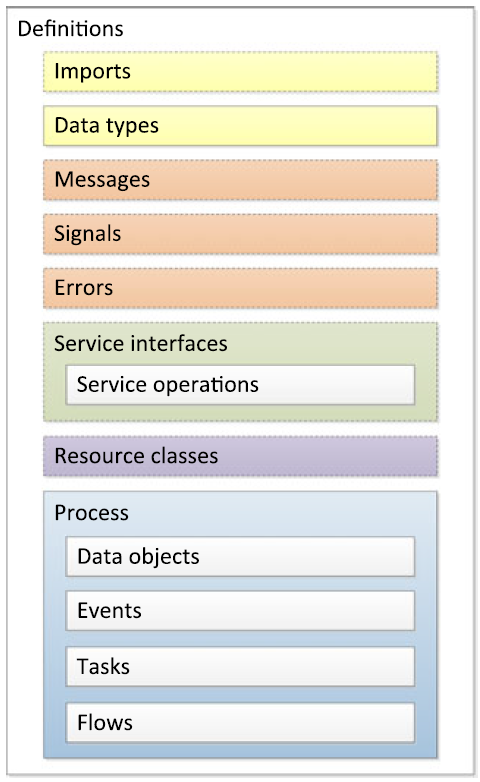
\includegraphics[width=0.3\columnwidth]{graphics/bpmn-schema}
		\caption{Structure of the BPMN format \cite{fundamentals}} 
		\label{fig:bpmn-schema} 
\end{figure}


\paragraph{Process Variables}~\\
In order to use data in different elements of our process, we need process variables that can be read, created and modified during the processes execution. Every Process variable has a \textbf{data type} that can either be simple (strings, integers, doubles, booleans, dates, times, ...) or complex (composed of other types). A complex Type needs to be described as an \gls{xsd}-Schema File.\\
\lstset{language=XML}
	\begin{lstlisting}[caption={The \gls{xml}-Schema Definiton for a complex type 'person'},captionpos=b]
<xs:element name="person">
	<xs:complexType>
		<xs:sequence>
			<xs:element name="name" type="xs:string"/>
			<xs:element name="address" type="xs:string"/>
			<xs:element name="city" type="xs:string"/>
			<xs:element name="country" type="xs:string"/>
		</xs:sequence>
	</xs:complexType>
</xs:element>
	\end{lstlisting}
\begin{lstlisting}[caption={An instance of the complex type 'person'},captionpos=b]
<person>
	<name>Dragana Sunaric</name>
	<address>Wiedner-Hauptstrasse 5</address>
	<city>1040 Wien</city>
	<country>Austria</country>
</person>
\end{lstlisting}


~\\The definition of common Errors, Messages and Escalations that are thrown or listened to by Events and Tasks are aslo part of the execution properties. Every Element has at least an \textbf{id} that identifies the given Element and a descriptive \textbf{name} of the element. \cite{bpmnstandard}
\paragraph{Messages}~\\
	\begin{lstlisting}
<message id="Message_ID" name="Message_NAME"/>
	\end{lstlisting}
\paragraph{Errors}~\\
Errors additionally have an \textbf{errorCode} that specifies the given Error. Events can listen for this specific error code and trigger when it is thrown.\\ 
	\begin{lstlisting}
<error id="Error_ID" name="Error_NAME" errorCode="Error_CODE"/>
	\end{lstlisting}
\paragraph{Escalations}~\\
Similar to errors, escalations additionally have an \textbf{escalationCode} that specifies the given Error and can be listened to by events. \\
	\begin{lstlisting}
<escalation id="Esc_ID" name="Esc_NAME" escalationCode="Esc_CODE"/>
\end{lstlisting}

\paragraph{Input and Output Variables}~\\
As mentioned earlier, Process Variables are active during the whole Process life-cycle. Apart from this data than can be accessed globally, it is also possible to define input and output values for each Task or Event in our process-model. These values are only visible within the Task or Event and have to be defined as an \gls{xsd}-Schema File (similarly to complex process variables). \cite{fundamentals}

\paragraph{Service Tasks}~\\
In order for service tasks to call external application or web-services, the interaction with the given service has to be defined in the process model. Connected services need to provide an service interface that describes the available service-operations and their parameters as well as return values. Service-operations can be synchronous, meaning the process instance waits for the operation to finish and to return a value or error code, or asynchronous, meaning the process does not wait for a response and carries on with the process after calling the service. Based on the service interface definition, input and output variables have to be defined for the service-call. The \gls{bpmn-engine} does this by copying the above mentioned Input values of the Task into the service call and if necessary, copy the output values of the service call into the output values of the Service task. \cite{fundamentals}





